\chapter{Experiential Learning\\ of Networking Technologies}
\vskip -15pt

\centerline{{\LARGE\sl Evolution of Socket Programming – Part I}}

\vskip 0.8cm

\begin{center}
{\large\uppercase{Ram P. Rustagi}}, 

\vskip -6pt

Department of CSE, KSIT Bengaluru 


\bigskip
{\large\uppercase{Viraj Kumar,}} 

\vskip -6pt

Divecha Centre for Climate Change, IISc Bengaluru

\end{center}

\vskip 2.3cm



\vfill
\newpage

\begin{multicols}{2}


\section{Introduction}
 
\vspace{-.2cm}
 
 We have studied both transport layers protocol i.e. TCP\cite{art1-key01} and UDP\cite{art1-key02}, in detail in the last few articles, and developed a basic understanding of working of transport layer. It is a communication enabling layer used by applications to exchange application level data. In this article, we will discuss socket programming and its evolution from a simple socket connection to a complex connection management especially when the need arises to attain high TCP performance.  In this article we will focus on TCP Socket programming only. UDP socket programming is simply a best effort delivery and socket implementation support does not impact the application communication performance.

\vspace{-.3cm}

\section{Basis of TCP Socket Programming}

\vspace{-.2cm}

Any network-based applications involve a pair of two entities, one that initiates request and another one that receives the request and responds back. In normal parlance, these are correspondingly called client and server. These two entities, for most practical purposes, reside in two different end systems and communicate to each other via an end to end logical network communication link, called socket. These two programs are most likely written by two different developers and thus need to follow application protocol standard, such as HTTP, FTP, SMTP, etc.  These applications either run over TCP or UDP, a decision taken by the application developer. In this article, we will discuss the development of application program using TCP and its evolution starting from a very simple request/response communication and gradually moving towards increasing complexity involving multiple concurrent communications, sharing or requests across many server processes, non-blocking socket communication and achieving performance improvement. As before, the hands-on exercises will be based on socket programs.  The example program will be in python language (the current most popular language, though socket programming was originally written in C) to explain the basics of socket programming and various states of socket enabling communication between client and server.

To working of socket programming and be explained with the analogy of two people \cite{art1-key03} residing in two different houses and need to communicate/meet with each other. Each house has a door that connects the house to outside world. The person residing in the house has full control over the house, but has little control over the outside world and need to follow the rules of outside world. House can be considered at par with application and outside world is like transport layer, which connects inside of a house to outside world. The door is analogous to a socket. Two houses can be neighbours to each other, across the street or even in different parts of the world. Consider that two people need to communicate with each other using a number of messages from each side and deploy an agent to deliver the messages in a reliable way. The agent receives the message at the door for first house, gets it delivered at the door of the other house and vice versa. The messages originate from the person in the house and consumed by the person in the other house.  These messages can follow any form and not necessarily one request and one reply. There can be number of messages from one side before receiving a number of messages or even none from other side. How, the person responds to each other’s message is up to them, but the job of the agency is to deliver these messages in a reliable way. The agency only ensures that whenever it delivers message to other end, these are delivered in-order, without any loss, corruption of duplication of messages. The working of agency is analogous to a TCP Connection. To ensure their continuous communication, two people first need to establish a connection using the agency, then carry on with sending and receiving the message and once over, release the agency.

Communication between two applications on two machines using sockets work in a similar way as described using above analogy. We will refer these two applications as client and server. The client process initiates the TCP connection to the server using a TCP socket, communicates with the server and then closes the connection. To enable this bidirectional communication, client first creates a socket (treated as flle descriptor in unix system), and connects it to server by specifying the server’s address (IP address and TCP port number). The server must have a created a socket beforehand to enable this connection i.e. accept the connection from the client. This connection setup involves 3-way handshake of TCP \cite{art1-key03}\cite{art1-key04}\cite{art1-key05} protocol which remains transparent to the client and server applications, which is then followed by data transfer in TCP ESTABLISHED state\cite{art1-key05}.  Finally, the connection closure involves handshake of 4 messages \cite{art1-key06}, which again remains transparent to applications. The interaction of client and server programs with network is implemented using socket library API calls. In this article, we first discuss usage of these API calls in a simple way and later on performance implications of socket API calls especially from the server perspective. 

\vspace{-.2cm}

\section{Socket Programming Approaches}

\vspace{-.2cm}

An introduction socket program is given in \cite{art1-key03} \cite{art1-key09}, and brief description of each API call can be found at \cite{art1-key08} and man pages \cite{art1-key10}.  The most common understanding of a simple client server interaction is shown in Figure~\ref{fig01} \cite{art1-key07} and elsewhere in the networking literature. At first, server creates a socket using \textit{socket()}, binds this socket to a well-known address (IP address and port number) using \textit{bind()}, informs the OS TCP stack about the number of connections that can be in queue waiting to be served by the server using \textit{listen()}, and then it accepts one connection at a time using \textit{accept()}. A typical analogy to understand these APIs can be understood by the following example. Consider the case that a number of students want to meet principal of a prospective college for admission purpose. The principal before coming to the college informs the office secretary/security to open the office, and this is equivalent to \textit{socket()} call. When principals enters the office and occupies the chair, this is equivalent to \textit{bind()} call. At this time, it does not mean that students can enter the office or meet the principal just because s/he is in the office. After a while, principal decides to allow students to come to the waiting room and wait there. This is equivalent to \textit{listen()} call. The number of chairs in the waiting hall corresponds to TCP listen queue size. If there are N chairs in the waiting hall, at most N students can wait. If there are M students (M$>$N) that come, then  M-N students have to go back and try again some time later. Still at this point, N students are in waiting room and most likely would meet the principal.
\begin{figure}[H]
\centering

\includegraphics[scale=1.2]{src/Figures/chap1/fig01.jpg}
\caption{Typical understanding of client server interaction}\label{fig01}
\end{figure}

After the principal completes any of the initial office work, and is willing to meet the students, s/he instructs the secretary to send one student inside the office. This is equivalent to \textit{accept()} call. The student can interact with principal as per the requirement and this will be equivalent to series of read()/write() calls. When one student enters the principal’s office, one vacancy is created in the waiting room and thus if any new student comes to meet principal, s/he can wait in the waiting room. It is possible for principal to permit multiple students (though one at a tie) to enter in his/her office and talk to them. Therefore, the number of students that can be inside the principal’s office will bear no correlation with number of students waiting in the waiting room. In the similar way, a server can concurrently communicate with multiple clients at the same time, and this number of concurrent communications is independent of number of clients waiting in the TCP listen queue. In brief, a TCP server program follows the path sequence \textit{bind()}, \textit{listen()}, and \textit{accept()} socket API calls, followed by required number of \textit{read()}/\textit{write()} calls. 

The invocation of socket API calls by a client follow a somewhat different path of socket API calls. Client create a socket (its endpoint of communication) using \textit{socket()} call. For a client to be able to talk to server, it must know IP address and port number of server application.  The client program provides these required parameters as part of connect() call to establish communication with server. The invocation of \textit{connect()} initiates the 3-wayTCP  handshake. Once the connection is established, it follows a series of \textit{write()}/\textit{read()} call to send data to and receive from the server and finally closes the TCP connection.

The communication flow in Figure~\ref{fig01} provides a conceptual understanding of TCP client server interaction and generally followed for a typical TCP based application communication. In this figure, it is shown that 3-way handshake is performed after the server issues \textit{accept()} call. However, in real life implementation of TCP stack, the communication flow for the server is slightly different and actual invocation of socket calls and interaction with a client is shown in Figure~\ref{fig02}. Using the earlier described analogy of students and principal interaction, this can be understood in the following way. When a student enters the waiting room, from all practical purpose, student is ready to communicate with principal, and this is equivalent to \textit{connect()} call. The student can start filling the required form which is needed by principal for the interaction. This is equivalent to client invoking \textit{write()} call even though principal hasn’t invoked the \textit{accept()} call yet i.e. hasn’t allowed the student to enter inside the office. Just because student has 

started providing information, it is expected that principal will call the student inside, but there is no guarantee that principal will call the student inside. It may happen that principal leaves the office for some reason (e.g. some emergency in college, or sudden call with university officials etc) which would result in students in the waiting room to leave the office i.e. unsuccessful communication. Same way, a client can invoke a number of \textit{write()} calls to send data and this data will reach the server side but will remain in the queue (like the filled form remains with the student) till server accepts the call and reads the data. Thus, a client can invoked \textit{connect()} to establish communication with the server immediately after server has invoked \textit{listen()}. From the client’s perspective, the connection is successful as shown in Figure~\ref{fig02}, and server can invoke the \textit{accept()} sometime later. Client can continue to send data even before server invokes \textit{accept()} or after it accepts the connection but hasn’t invoked the read(). This call acceptance mechanism on server side is the primary difference between Figure~\ref{fig01} and Figure~\ref{fig02}. In the discussion below we will study this behavior of the server-side TCP connection management w.r.t. multiple concurrent clients and explore the functionality of socket APIs.

\begin{figure}[H]
\centering
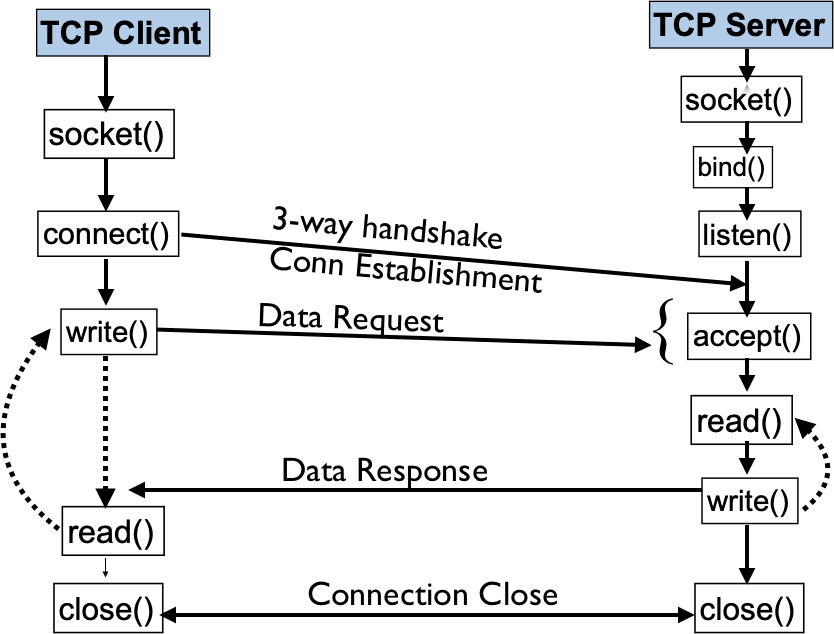
\includegraphics[scale=1.2]{src/Figures/chap1/fig02.jpg}
\caption{Practical working of TCP sockets interaction}\label{fig02}
\end{figure}


\section{A Server with Just One Client Connection}

A very simple TCP server program would correspond to accepting request from only a single client, serve these requests and then exit. A simple working of such a communication can be experienced using \texttt{netcat as a server (nc -1 $<$port)}. This would run a TCP server binding on the specified port with option -1 and all the IP Addresses associated with server machine. The netcat server accepts a single client request and as long as client is connected it will receive the message from client and display the same on terminal window. When client closes the connection, this simple server would close the connection and exit as well. However, to develop a better understanding of using \textit{bind(), listen()} and \textit{accept()} call, consider a simple python program \texttt{tcp\_server01.py} \cite{art1-key11}, and the required code snippet is shown in left column of Table~\ref{fig03}. This code is very similar in behaviour to \texttt{netcat (nc)} server, where client connects to server on the known IP address and port number, sends messages and when client closes the connection, the server program also closes the accepted connection and exits. By default, in all our exercises we will \texttt{netcat(nc)} as the client program which will be invoked as \textbf{“nc <server IP> <server port>”}, unless specified otherwise.

\end{multicols}

\setcounter{section}{0}
\begin{table}[H]
\centering
\caption{Server program that accepts 1 client request}\label{fig03}
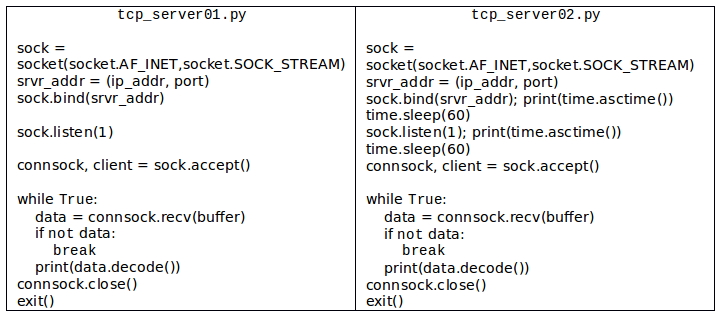
\includegraphics[scale=3.05]{src/Figures/chap1/fig03.jpg}
\end{table}

\begin{multicols}{2}
To understand interdependencies between \textit{bind()}, \textit{listen()} and \textit{accept()}, consider the code snippets of modified program \texttt{tcp\_server02.py} \cite{art1-key11} as shown in right column of Table~\ref{fig03}. The server invokes \textit{listen()} 60 seconds after its binds to its port number. So, even though program is running, the TCP stack on the server machine has no information if server program would service any requests and if any clients can be put in the queue till \textit{listen()} is invoked by the server. Thus, till \textit{listen()} is invoked by the server, if a client tries to connect to the server, the connection attempt will be unsuccessful. The server program with TCP port number 9999 (default port number value used by the server programs) is started at 15:18:26 as shown by $2^{\rm{nd}}$ line in right column of Table~\ref{fig04}. Netcat program \cite{art1-key12} is used as a client to connect to this server. As shown in left column of Table~\ref{fig04}, first two attempts at time 15:18:31 and 15:19:15 are terminated till time server executes \textit{listen()} call (Line 5 in right column of Table~\ref{fig03}) at 15:19:26 (3rd line in right column of Table~\ref{fig04} . The next attempt after that is successful (line 4 in left column Table~\ref{fig04}). 
\end{multicols}

\begin{table}[H]
\centering
\caption{Network implication of delayed listen(), accept()}\label{fig04}
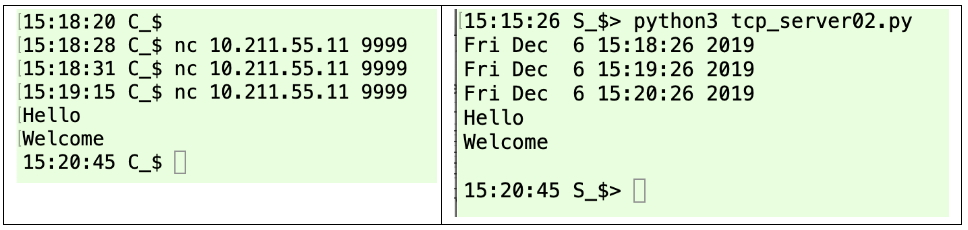
\includegraphics[scale=2.28]{src/Figures/chap1/fig04.jpg}
\end{table}

\begin{table}[H]
\centering
\caption{Status of network connection at Server Machine}\label{fig05}
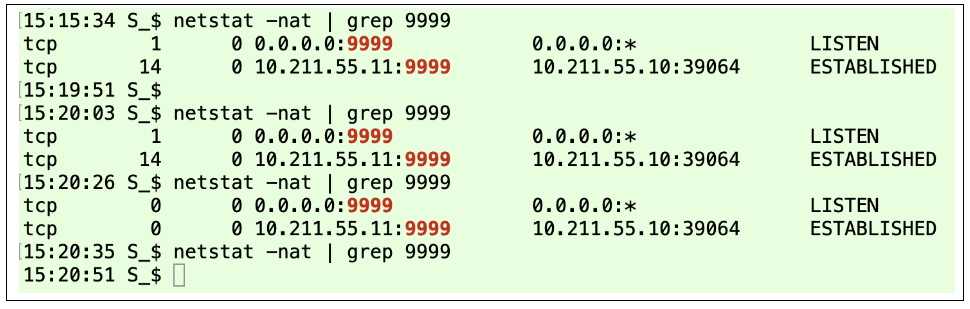
\includegraphics[scale=2.25]{src/Figures/chap1/fig05.jpg}
\end{table}

\begin{multicols}{2}

At this stage server program has not accepted the client connection. The server program accepts the connection 60 seconds after the \textit{listen()} call (line 7, Table~\ref{fig03}). However, from the client and system perspective, the TCP connection is established at time 15:19:51 as shown by first 4 lines in Table~\ref{fig05}. Since connection is established from client’s view, it can send data on this connection as shown by lines 5-6 in clients window (column 1 Table~\ref{fig04}). This data (\texttt{“hello + $\backslash$n + wecome + $\backslash$n”} ; a total of 14 characters)  has reached the server and is in the queue of this connection at server side as shown by $2^{\rm{nd}}$ field of line  3 and line 7 in Table~\ref{fig05}.

When client accepts by invoking accept() the request 60 seconds after \textit{listen()} at time 15:20:26 (line 4 in right column of Table~\ref{fig04}) and reads the data, queue for this connection is cleared as shown by queue size of 0 ($2^{\rm{nd}}$ field of line 10 in Table~\ref{fig05}). When client exits at time 15:20:45, the connection is closed on the server side as well and network connection status shows no connection at time 15:20:51 (last two lines in Table~\ref{fig05}). 

In general, a server program is expected to run forever and should be able to serve multiple clients. Thus, the next stage of server program should evolve to a state where it runs forever, and whenever one client connection closes, it should accept request from next subsequent client and so on. The number of clients that remains in the queue is determined by the parameter value of \textit{listen()} API call. If a new client connects when the queue is full, this connection request would be rejected and client program would exit. To study the impact of queue size, run the server program \texttt{tcp\_server02.py}\cite{art1-key11} and connect to this server with multiple client programs. When listen queue becomes full, TCP stack on server simply ignores TCP SYN (connection setup request\cite{art1-key03}\cite{art1-key13}) and does not respond at all. The client will retry the connection by resending TCP SYN packets a pre-configured number of times, which is identified by system configuration and tuning parameter \texttt{net.ipv4.tcp\_syn\_retries} value, which is default of 6 on Ubuntu. As per TCP timeout implementation, each time it sees a timeout, it doubles the timeout value and thus for our purpose of studying listen queue size behaviour, it is recommended to set this value to 1 (use the command \texttt{sudo sysctl -w net.ipv4.tcp\_syn\_retries=1}) on the client machine. Further, as per Linux system implementation of listen socket call \cite{art1-key12}, the real maximum queue length is 1.5 times more than the value specified in the \textit{listen()} call. As server program invokes \textit{listen(1)}, the queue size is going to be more than 1, and observed value is 2.

To study the behaviour of \textit{listen()} and backlog of queues, modify the server program just to put a delay of 60 seconds between \textit{listen()} and \textit{accept()}. There is no need to have any delay between \textit{bind()} and \textit{listen()}. When we run this new server program \texttt{tcp\_server03.py}, and then connect 3+ clients to it (with \texttt{syn\_retries} value set to 1) within 60 seconds of starting of the server program, it should result in first two clients connecting successfully to server and $3^{\rm rd}$ client program being unsuccessful after retries. This is shown in Table~\ref{fig07} (top row, first two lines), where server program starts 15:28:22, executes \textit{bind()}, \textit{listen()} immediately but waits for 60 seconds before executing \textit{accept()}. Invocation of client programs (nc) is shown in Table~\ref{fig06}, where clients in left column are successful whereas clients in right columns are unsuccessful, which are invoked at 15:28:32 and 15:28:53. The TCP server shows tow connections in ESTABLISHED state (first 10 lines in bottom row of Table~\ref{fig07}) a time 15:28:36 as well as at time 15:28:46.
\end{multicols}


\begin{table}[H]
\centering
\caption{Concurrent client requests to a single server}\label{fig06}
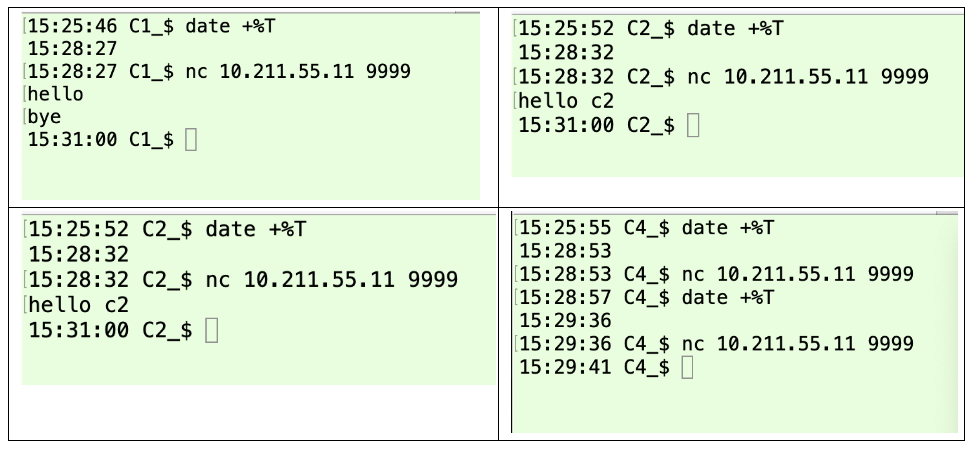
\includegraphics[scale=2.26]{src/Figures/chap1/fig06.jpg}
\end{table}

\begin{multicols}{2}

At time 15:29:32, server invokes \textit{accept()}, and when a new clients connects after this time, this $3^{\rm rd}$ client is connected, number of connections in ESTABLISHED state becomes 3 as shown in (lines 11-16, bottom row of Table~\ref{fig07}. The line 13 size of listen queue is 2 corresponding to two connections pending to be accepted, and line 16 shows queue size to be 9 implying that a client has sent 9 bytes of data which needs to be read by server. When $4^{\rm th}$ client, as shown in lines 5-6 in bottom row right column of Table~\ref{fig06} tries to connect at time 15:29:36, the connection fails. The bottom row shows the output of tcpdump which demonstrates that two TCP SYN packets are received (first one corresponding initial connection request and $2^{\rm nd}$ one corresponding to retry) and no response is given by server.

Once the server accepts a connection request from a client (after 60 seconds of listen), the queue for pending connections become 1 less and thus any new client request will be accepted and it will show ESTABLISHED state. Other client connection requests will be ignored as queue has become has full. Table ?????? shows three client requests in connected state, where as $4^{\rm th}$ client is unsuccessful.
\end{multicols}



\begin{table}[H]
\centering
\caption{Single request handling Server connection status}\label{fig07}
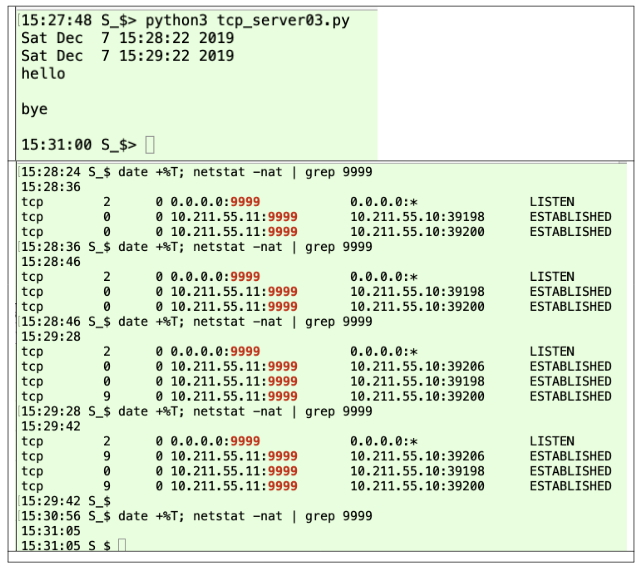
\includegraphics[scale=3.45]{src/Figures/chap1/fig07.jpg}
\end{table}

\begin{multicols}{2}

when first client exits (pressing Ctrl-D in nc), the connection is closed,  and exits at time 15:31:00, the server also exits after serving one client. This is because, the server program (\texttt{tcp\_server03.py}) accepts only one connection, and exits after the first connection is closed. The last two lines of bottom row of Table~\ref{fig07} shows no connections at time 15:31:05. The other clients requests are simply terminated without any actual communication accepted by the server. From the client perspective, this is bit puzzling since client sees the connection in ESTABLISHED state, but has no clue why connection was terminated.

\end{multicols}


\begin{table}[H]
\centering
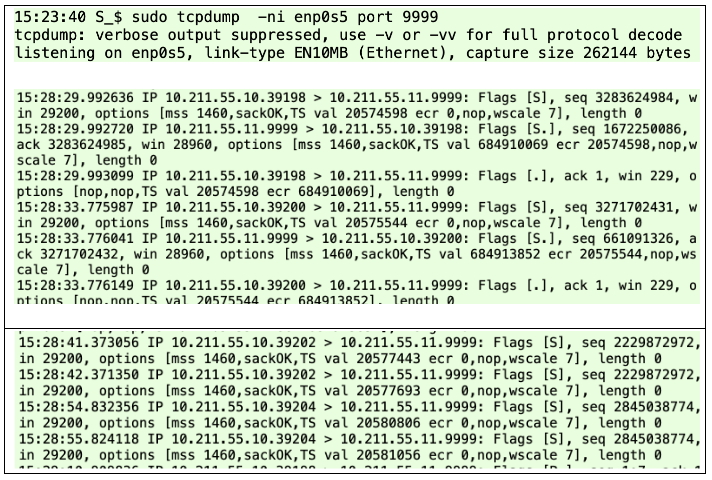
\includegraphics[scale=3.06]{src/Figures/chap1/fig08.jpg}
\end{table}

\begin{multicols}{2}

\setcounter{section}{4}
\section{A Perpetual Server with Just One Client Connection at a time}

A natural extension to server programs to accept new connection after it complete its interaction with currently client. This will involve and perpetual running loop that would accept a new connection, service the client and then go back to accept connection from the new client. A sample snippet of such a code from server program \texttt{tcp\_server04.py} \cite{art1-key04} is shown in Table~\ref{fig09}. 

\end{multicols}


\begin{table}[H]
\centering
\caption{Perpetual server with one connection at a time}\label{fig09}
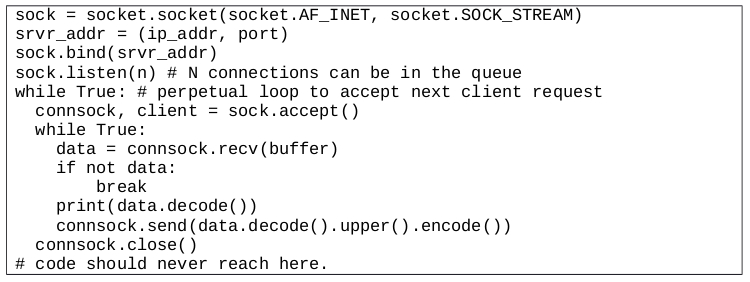
\includegraphics[scale=2.92]{src/Figures/chap1/fig09.jpg}
\end{table}

\begin{multicols}{2}
This server program works fine to deal with any number of clients. However, such a server suffers from severe performance issues. Since sever program is handling one client at time, the other clients which are in queue have to wait for a much longer time to be able to get any service from the server. Such a behaviour is not acceptable in real life situations. Consider a bank website that works in this way i.e. serves only customer login and associated interaction one at time, then all other customers who are waiting in the queue will get totally frustrated and would not use the website again at all. Thus, for an effective web server, it is of paramount importance to serve the multiple clients concurrently.

\section{A Perpetual Server with Multiple Concurrent Connections}

The well know webservers, such as Apache, nginx etc.”, serve hundreds of thousands of concurrent clients. These web servers provide a lot more functionality than just managing concurrent TCP connections and have evolved into a complex implementation to serve these clients efficiently. In this article, we take a simplistic view from TCP perspective on how these concurrent clients can be served. There are many possibilities to serve concurrent client and we will start from a very basic simple approach though inefficient to somewhat complex approach from implementation perspective but efficiently handles concurrent connections.

The most simplistic approach would be to create a separate process for each client. Thus, a parent process starts and waits for new client request. Whenever, client connects, it spawns a new child process and it is that child process that is dedicated to serve the client. Once the client closes the connection, this child process exits. A simple code snippet of simple program \texttt{tcp\_server05.py} \cite{art1-key04} using this approach is shown in Table~\ref{fig10}.
\end{multicols}


\begin{table}[H]
\centering
\caption{Server spawnin child process for each client}\label{fig10}
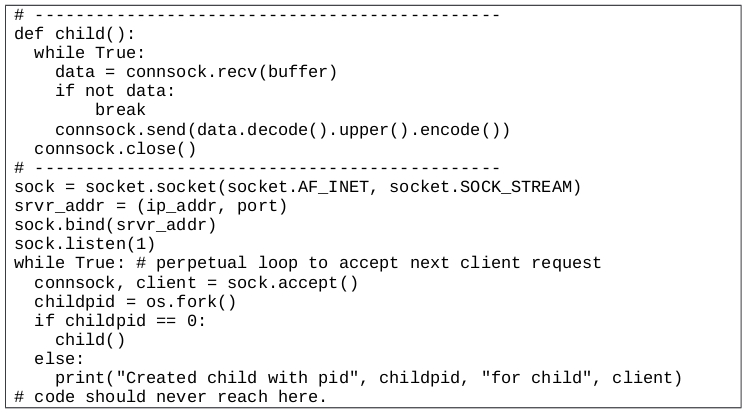
\includegraphics[scale=2.92]{src/Figures/chap1/fig10.jpg}
\end{table}

\begin{multicols}{2}

The inefficiency of this approach lies in the fact that a new process is to be created for each client. Creation of a new process consumes significant amount of OS resource both in terms of memory and compute time, and this approach can work well for a limited number of concurrent clients, few hundreds or possibly thousand. When number of concurrent client exceeds thousands, the process scheduling by operating system will itself take a heavy toll on the system and bring down the system performance. Thus, this approach is not scalable. Another common problem that developers often face in this approach corresponds to zombie or defunct process. This problem arises when a child process exits, but parent does not wait for the exit status of a child process. As per unix process implementation, a parent must wait for child process to exit, receive the exist status of child process and take necessary action which in most case is none. A zombie process though remains idle and does not consume CPU time, but does consume process table resources of the operating system. So if such a server has run for some time, and has received N number of new client connections, there will be N number of zombie processes in the system and at some point in time, system will run out resources (process table memory space). A simple solution to this issue is parent must invoke the waitpid() method for exited child process. A sample snippet of server program\textit{tcp\_server05b.py} is shown in Table~\ref{fig11}. The method waitpid() is invoked with first parameter as -1 implying any of the child, and $2^{\rm nd}$ parameter as WNOHANG implies that his method is non-blocking. If a child has existed, this method will return the exit status of that child else return error -1.
\end{multicols}


\begin{table}[H]
\centering
\caption{Modified sever code waiting for child to exit}\label{fig11}
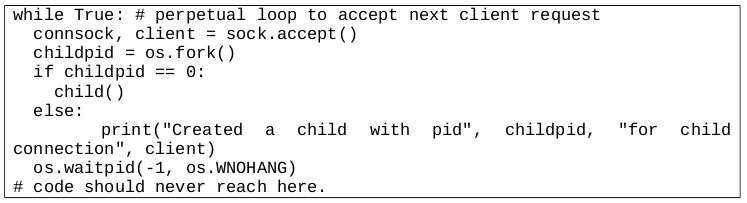
\includegraphics[scale=2.92]{src/Figures/chap1/fig11.jpg}
\end{table}

\begin{table}[H]
\centering
\caption{server creating predefined number of child processes}\label{fig12}
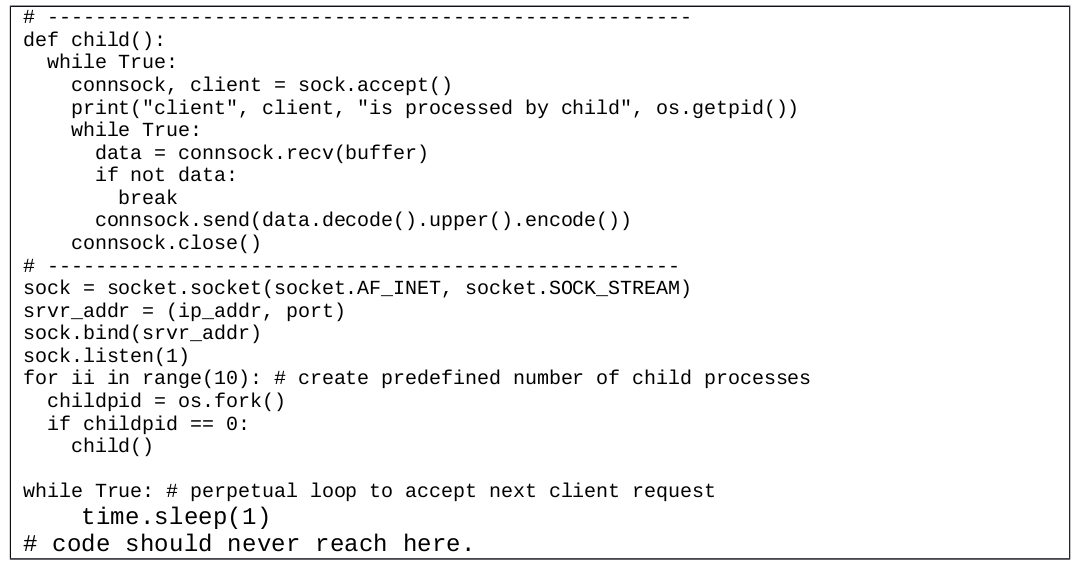
\includegraphics[scale=2]{src/Figures/chap1/fig12.jpg}
\end{table}

\begin{multicols}{2}
One possibly way to improve the above approach is to create a fix number of child processes beforehand and new client can be assigned to any of the free child process. The sample snippet code of program \texttt{tcp\_server06.py}\cite{art1-key04} is shown in Table~\ref{fig11}, which creates 10 children process beforehand. The parent process remains idle for all practical purposes. Each process invokes its own \textit{accept()} and it is up to the OS to pick the child process to which the new incoming connection request should be assigned.  Thus, the approach of distributing the connection also has been from application domain to system domain. This approach certainly helps saves OS overhead of creating a process, and thus performs better than earlier approach.

However, this poses a new problem. When the number of clients exceeds the total number of pre-created children processes plus the required queue size and those children will be denied connection request from the client. A simple solution would be that each client communicates to parent whenever it receives a new request as well as when the connection is closed. This parent knows how many clients are being served and thus, when it sees the number of clients is approaching the number of pre-created children processes or number of free children processes have fallen below a specified threshold, it can create more child process. Thus, this entails some amount of communication between child and parent process and parent process needs to do some book keeping of creating new children or even kill idle children if they are too many. A further improvement can be done by using the threads instead of child process. This way OS scheduling overhead is lower compared to that of dealing with equal number of child processes. But writing a thread safe code is another challenge that developer needs to deal with and not many programmers are efficient in writing multi thread robust code. However, the problem of scaling still persists and only a limited number of clients can be served using this approach. 
\end{multicols}

\begin{table}[H]
\centering
\caption{Concurrent connections handling using select() call}\label{fig13}
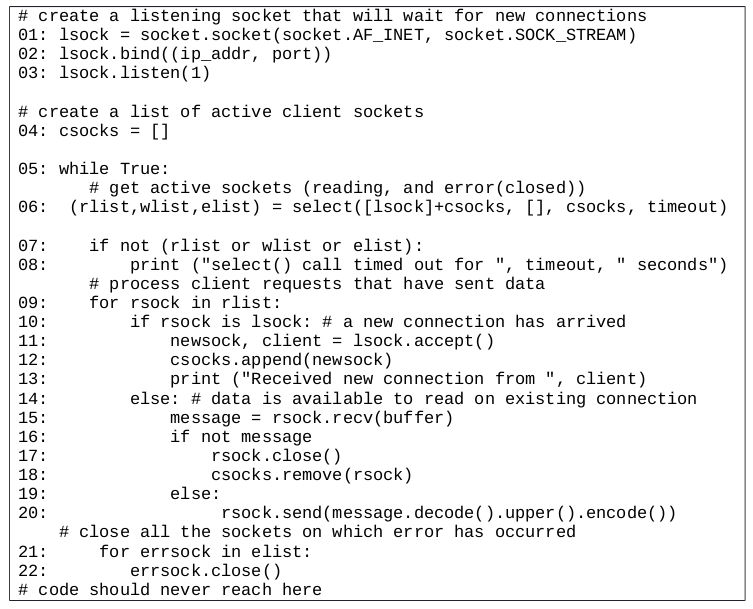
\includegraphics[scale=2.95]{src/Figures/chap1/fig13.jpg}
\end{table}

\begin{multicols}{2}

\section{Serving Multiple Concurrent Connections using \textit{select()}}

For an efficient server process implementation, it is desirable to avoid create one child process for each new client, and avoid pre-forked approach of creating a specified number of children process, but should be able to concurrently handle multiple clients. In general, when N clients are connected to the server, not all of them communicate with server at the same time. For example, consider N browsers accessing a web server. When a web page is downloaded, user will take time to glance over (read) it there will be significant time gap before the next request is made to the web server. Thus, at any point of time, only a few clients would be concurrently sending the requests to web server and receiving the response. A naïve approach to efficiently deal with situation is a single threaded process, which maintains all the connected socket in an array and continuously check which of the socket in the array has data received from the associated client and respond accordingly. The socket library call \texttt{select()} (C language: \cite{art1-key14}, python 3 documentation: \cite{art1-key15}) exactly provide such a functionality. The method has its input as array of sockets to check for which sockets have data availability and return back the list of these active sockets to application. For each of these active sockets i.e. the clients who have sent data, server programs reads the data and communicates accordingly. The original socket also is part of read list. Whenever, a new client connects, this socket is considered equivalent to read and needs to checked for accordingly. The server program using the select() API call is given in \texttt{tcp\_server07.py} and basic code snippets highlighting the use is given in Table~\ref{fig13}.

This program is a simplified example of concurrent client connections handling limited to reading data from the client requests and does not show the use of select() for writing data on these sockets. The select() requires 4 parameters: a) first is list of sockets on which data can be sent by clients, b) second is the list of sockets where data can be written, but given empty list in this example, c) third parameter is list of sockets which have been closed by the clients(), and d) the last parameter is timeout. This timeout is used for select() call to return if no active sockets are found from the 3 lists. New arriving connection processing is shown in lines 10-13. The data from active clients is shown in lines 14-15, 19-20. The lines 16-18 shows the connection processing when client closes the connection.

The approach using select() performs better than earlier approaches of creating multiple threads/processes. The select() call is based on unix system call \cite{art1-key14}, which in general has a default limit of 1024 connections as this is based on bit size. Thus, a server using select() is generally limited to handling 1024 concurrent clients. In today’s internet, a server needs to deal with large number of connections and thus select() in sufficient for this purpose. This limit of 0f 1024 concurrent clients is overcome by two other socket API calls, namely poll() and epoll(), which we will discuss in the next article. The major difference between poll() and select() is basically internal implementation details and former is more efficient than latter, in addition to former supports more than 1024 clients. Epoll() is event based implementation and even more efficient than poll().

\section{summary}

We have discussed the progression of approaches for a TCP server program to handle multiple concurrent clients. The server processing starts from server processing one client at a time and thus causes significant delays to waiting clients, leading to a poor user experience. The next approach is to create one child process (or thread for more efficient processing) which is a simplified approach as each child process separately deals with each client. This makes the programming simple as developer does not have to write code for managing multiple sockets. This approach works fine though inefficient since child process creation results in high overhead for underlying OS. The alternative approach is to create a pre-configured number of children processes (or threads()).This avoids the overhead of process creation but imposes a limit on number of client processes that can be served. A better efficient approach is to make use of select() to serve multiple concurrent clients, which again has efficiency issues and limit on number of concurrent clients to be 1024 (can be changed by recompiling the linux kernel). More efficient processing is provided by use of poll() and epoll() calls.

An practical example of server side porgram using the above discussed approach is more popular Apache web server \cite{art1-key16}.  The web server supports preforked model where a number preconfigured child server processes are created. The parent process manages the size of server pool and creates or kill child processes as required. The web server also supports a worker model where the child process creates multiple threads to process multiple clients. This is more efficient than preforked approach. Finally, the most efficient supported implementation corresponds to event model, which implements a hybrid multiple process, multi-threaded server. This consumes less resources compared to worker model. The event model is supported on unix variants and not on windows. Another, more popular and widely deployed web server is nginx \cite{art1-key17}, which by default is single threaded server per CPU core. It basically, provides a most efficient implementation using epoll() mechanism.

\section{Experiential Exercises}

The complete code of server programs as discussed in the article for both python and C language (not discussed in the article) can be access from \cite{art1-key11}. The setup for these exercises a simple setup of two machines connected on a network, one acting as a client and other server. The server machine should be running Linux operating systems, where client could be any one. For the client application, netcat (nc) \cite{art1-key12} would be used, which is available by default on Linux and macOS, but need to be installed on Windows OS. On the server, it python scripts would be invoked. As a place holder, the IP Address of client and server are respectively taken as 10.211.55.2/24 and 10.211.55.11/24. The server program \texttt{tcp\_server$<$NN$>$.py} by default uses the port number 9999 and can be changed to other value with option -p. On the client machine, configure the number SYN retries to 1. On linux based clients, this can be done with \texttt{sudo sysctI -w net.ipv4.tcp\_syn\_retries=1}.

\setcounter{section}{0}
\section*{Exercise \thnum{1}\label{chap1-exe01}}

\textbf{Topic: TCP Server handling a single client with multiple clients queueing.}

\begin{itemize}
\item[a.] Invoke the server program \texttt{tcp\_server01.py} on server machine. This server accepts only one client request and exits after client closes the connection.

\item[b.] On the client machine(s) [can use more than 1 client machine as well], invoke netcat in 3 different terminal windows as below

\texttt{nc 10.211.55.11 9999}

\item[c.] All 3 clients would be connected. From each of the client send some data e.g. \texttt{“Hello 1”, “Hello 2”, “Hello 3”}, etc.

\item[d.] On the server, check connection status as below. 

\texttt{Netstat -natp | grep 9999}

\item[e.] It should show 3 connections in ESTABLISHED state similar to that shown in Table~\ref{fig07}. The data from first client will be shown on server terminal, data from other two clients will be shown as queued in $2^{\rm nd}$ column of \texttt{netstat} output.
\item[f.] Exit from the first client. Check the connection state on the server. All 3 connections would be closed and server program would also exit.
\item[g.] Repeat the above exercise using the server programs \texttt{tcp\_server02.py} and \texttt{tcp\_server03.py} instead of \texttt{tcp\_server01.py} and analyze the server program behaviour. The former will demonstrate the use of \textit{bind()} and \textit{listen()}, and latter will exhibit the working of \textit{listen()} and \textit{accept()}.
\end{itemize}

\vspace{-.2cm}

\textbf{Learning:} Handing of multiple client connections and queueing of these on account of TCP listen().

\vspace{-.35cm}

\section*{Exercise \thnum{2}\label{chap1-exe02}}

\textbf{Topic: Perpetual TCP server handling one client at a time}

\begin{itemize}

\item[a.] Invoke the server program \texttt{tcp\_server04.py} on server machine. This server accepts one client request at a time, accepts the next client request when previous client closes the connection. Thus, the server program runs from ever.

\item[b.] On the client machine(s), invoke netcat in 3 different terminal windows as below

\texttt{nc 10.211.55.11 9999}

\item[c.] All 3 clients would be connected. From each of the client send some data e.g. \texttt{“Hello 1”, “Hello 2”, “Hello 3”}, etc.

\item[d.] On the server, check connection status as below.

\texttt{Netstat -natp | grep 9999}

\item[e.] It should show 3 connections in ESTABLISHED state similar to that shown in Table~\ref{fig07}. The data from first client will be shown on server terminal, data from other two clients will be shown as queued in $2^{\rm nd}$ column of \texttt{netstat} output.

\item[f.] Exit from the first client. Server would proceed to accept next connection and display the data from second client. Accordingly verify the number of ESTABLISHED connections using \texttt{netstat}.

\item[g.] Connect few more clients than permitted by listen queue size and verify that connections are rejected and when queue size is exceeded.

\end{itemize}

\textbf{Learning:} Handing of multiple client connections and processing of these by server one at a time.

\section*{Exercise \thnum{3}\label{chap1-exe03}}

\textbf{Topic: Perpetual TCP Server handling concurrent clients using creating one child process per client}

\begin{itemize}

\item[a.] Invoke the server program \texttt{tcp\_server05.py} on server machine. This server accepts one client request at a time, accepts the next client request when previous client closes the connection. Thus, the server program runs from ever.

\item[b.] On the client machine(s), invoke netcat in N (e.g. 3 or more) different terminal windows as below

\texttt{nc 10.211.55.11 9999}

\item[c.] All these clients would be connected. From each of the client send some data e.g. \texttt{“Hello 1”, “Hello 2”, “Hello 3”}, etc.

\item[d.] On the server, check connection status as below and number of server processes. 
 
 \texttt{netstat -natp | grep 9999}
 
 \texttt{ps -efw | grep tcp\_server05}
 
\item[e.] It should show N connections in ESTABLISHED state and N+1 process 1 corresponding to parent process, and 1 child process for each client. The data from all the client will be shown on server terminal. Since each client is served actively and not waiting at all, no data should be shown in queue i.e. $2^{\rm nd}$ column of \texttt{netstat} output should show value 0.

\item[f.] Exit from some clients e.g. K clients closes the connection and initiate new connections from M other clients. The total number of process that should be equal to 1+N+M. Essentially, even though client has closed the connection, the corresponding server child process continue to remain in the process list (which essentially becomes a zombie process).

\item[g.] Abort the main server parent process (e.g. Ctrl-C on server window) and where server program is running. This will clean out server processes and also all client netcat process will also exit because nc exits when connection is closed.

\item[h.] Repeat the above experiment with variant \texttt{tcp\_server05b.py} of this server program. Verify that at any time, number of server child processes correspond to number of connected clients.

\end{itemize}

\textbf{Learning:} Handing of multiple client connections with a dedicated server child process and clean-up of zombie processes.

\section*{Exercise \thnum{4}\label{chap1-exe04}}

\textbf{Topic:  Perpetual TCP Server handling multiple concurrent clients using pre-created child process.}

\begin{itemize}

\item[a.] Invoke the server program \texttt{tcp\_server06.py} on server machine. This server program creates fixed number (e.g. 3) child processes. The program, by default, creates 10 children processes. Use option \texttt{-c <N>} to specify count of children processes.

\item[b.] On the server machine, verify number of server processes to be \texttt{N+1}, 1 parent, \texttt{N} children.

\texttt{ps -efw | grep tcp\_server06}

\item[c.] Each of child process executes \textit{accept()} on the single listening socket shared by all. Thus, whenever a new client connection request arrives, OS directs the incoming connection to one of the child process which accepts and process the client requests.

\item[d.] On the client machine(s), invoke netcat in N (e.g. 3 or more) different terminal windows as below

\texttt{nc 10.211.55.11 9999}

\item[e.] All these clients would be connected. From each of the client send some data e.g. \texttt{“Hello 1”, “Hello 2”, “Hello 3”}, etc.

\item[f.] On the server, check TCP connection status.  Verify it should be equal to number of clients.

\item[g.] Invoke few more clients (nc) to exceed queue size. Verify the number of TCP connections in ESTABLISHED state to be equal to number of server children processes plus listen queue size, and other clients would exit after connection timeout.
\end{itemize}

\textbf{Learning:} Understand limitations on number of clients that can be concurrently server using pre-forked children processes.

\section*{Exercise \thnum{5}\label{chap1-exe05}}

\textbf{Topic: Perpetual TCP Server handling multiple concurrent clients using \textit{select()} call.}

\begin{itemize}

\item[a.] Repeat the first six steps of Exercise~\ref{chap1-exe04} with replacing the server program \texttt{tcp\_server06.py} by \texttt{tcp\_server07.py}.

\item[b.] Verify that number of ESTABLISHED connections are equal to number of clients communicating with server. All the clients can concurrently communicate with the server.

\item[c.] Verify that there is only a single server process running on the server.

\item[d.] Activate few more clients and these will connect to server successfully and communicate with it. Try as many clients as would like to. The single threaded server process can handle up to 1024 clients concurrently.
\end{itemize}

\textbf{Learning:} Understand general implementation of an efficient server side program that can handle 1000+ concurrent clients.

\section*{Appendix}

\begin{thebibliography}{99}
\bibitem{art1-key01} RFC 793, “Transmission Control Protocol “, Information Sciences Institute, USC, CA, Sep 1981, 

\url{https://tools.ietf.org/html/rfc793. Last accessed May 2019.}

\bibitem{art1-key02} RFC 791, “User Datagram Protocol”,.....

\bibitem{art1-key03}Kurose, Ross, “Computer Networking: A Top Down Approach”, section 3.5.5, $6^{\rm th}$ edition, Pearson,

\bibitem{art1-key04} Ram Rustagi, Viraj Kumar, “Understanding Basics of Transport Layer”, ACCS journal of Computing and Communications, Vol 2, Issue 3, September 2018

\url{https://journal.accsindia.org/experiential-learning-of-networking-technologies-understanding-transport-layer-basics/,}

last accessed Aug 2019

\bibitem{art1-key05} Ram Rustagi, Viraj Kumar, “Understanding TCP States Part - I”, ACCS journal of Computing and Communications, Vol 2, Issue 4, Decemeber 2018,

\url{https://journal.accsindia.org/experiential-learning-of-networking-technologies-understanding-tcp-states-part-1,}

last accessed Dec 2019.

\bibitem{art1-key06} Ram Rustagi, Viraj Kumar, “Understanding TCP States Part - II”, ACCS journal of Computing and Communications, Vol 3, Issue 1, March 2019,

\url{https://journal.accsindia.org/experiential-learning-of-networking-technologies-understanding-tcp-states-part-2/,}

last accessed Dec 2019.
\bibitem{art1-key07} \url{ftp://www.cs.uregina.ca/pub/class/330/Sockets/sockets.html,}

 last accessed Dec 2019

\bibitem{art1-key08} Linux Socket programming: 

\url{http://www.linuxhowtos.org/C_C++/socket.html}

\bibitem{art1-key09} Basic description of socket programming,

\url{http://inst.eecs.berkeley.edu/~ee122/fa09/notes/03-SocketProgrammingx6.pdf}

\bibitem{art1-key10} Linux man page for socket APIs,

 \url{http://man7.org/linux/man-pages/man2/socket.2.html}

\bibitem{art1-key11} Source code of server socket programs.

\url{https://github.com/rprustagi/EL-Evolution-of-Server-Socket-Programming}

\bibitem{art1-key12} Netcat (nc) command utility,

\url{http://manpages.ubuntu.com/manpages/xenial/man 1/nc.traditional.1.html},

last accessed December 2019. 

\bibitem{art1-key13} Ubuntu man page for listen socket call.

\url{http://manpages.ubuntu.com/manpages/bionic/man2/listen.2freebsd.html}

\bibitem{art1-key14} Man page of select() api,

\url{http://manpages.ubuntu.com/manpages/trusty/man2/select.2.html,}

last accessed Dec 2019.

\bibitem{art1-key15} Documentation of python 3 select API, 

\url{https://docs.python.org/3/library/select.html}, 

last accessed Dec 2019.

\bibitem{art1-key16} Apache web server multi processing module,

\url{http://httpd.apache.org/docs/2.4/mpm.html},

 last accessed Dec 2019.
 
\bibitem{art1-key17} Nginx web server, 

\url{http://nginx.org/en/},

last accessed Dec 2019.

\end{thebibliography}
\end{multicols}


